\begin{figure}[htbp]
    \centering
    \subfigure[The Transformer block]{
        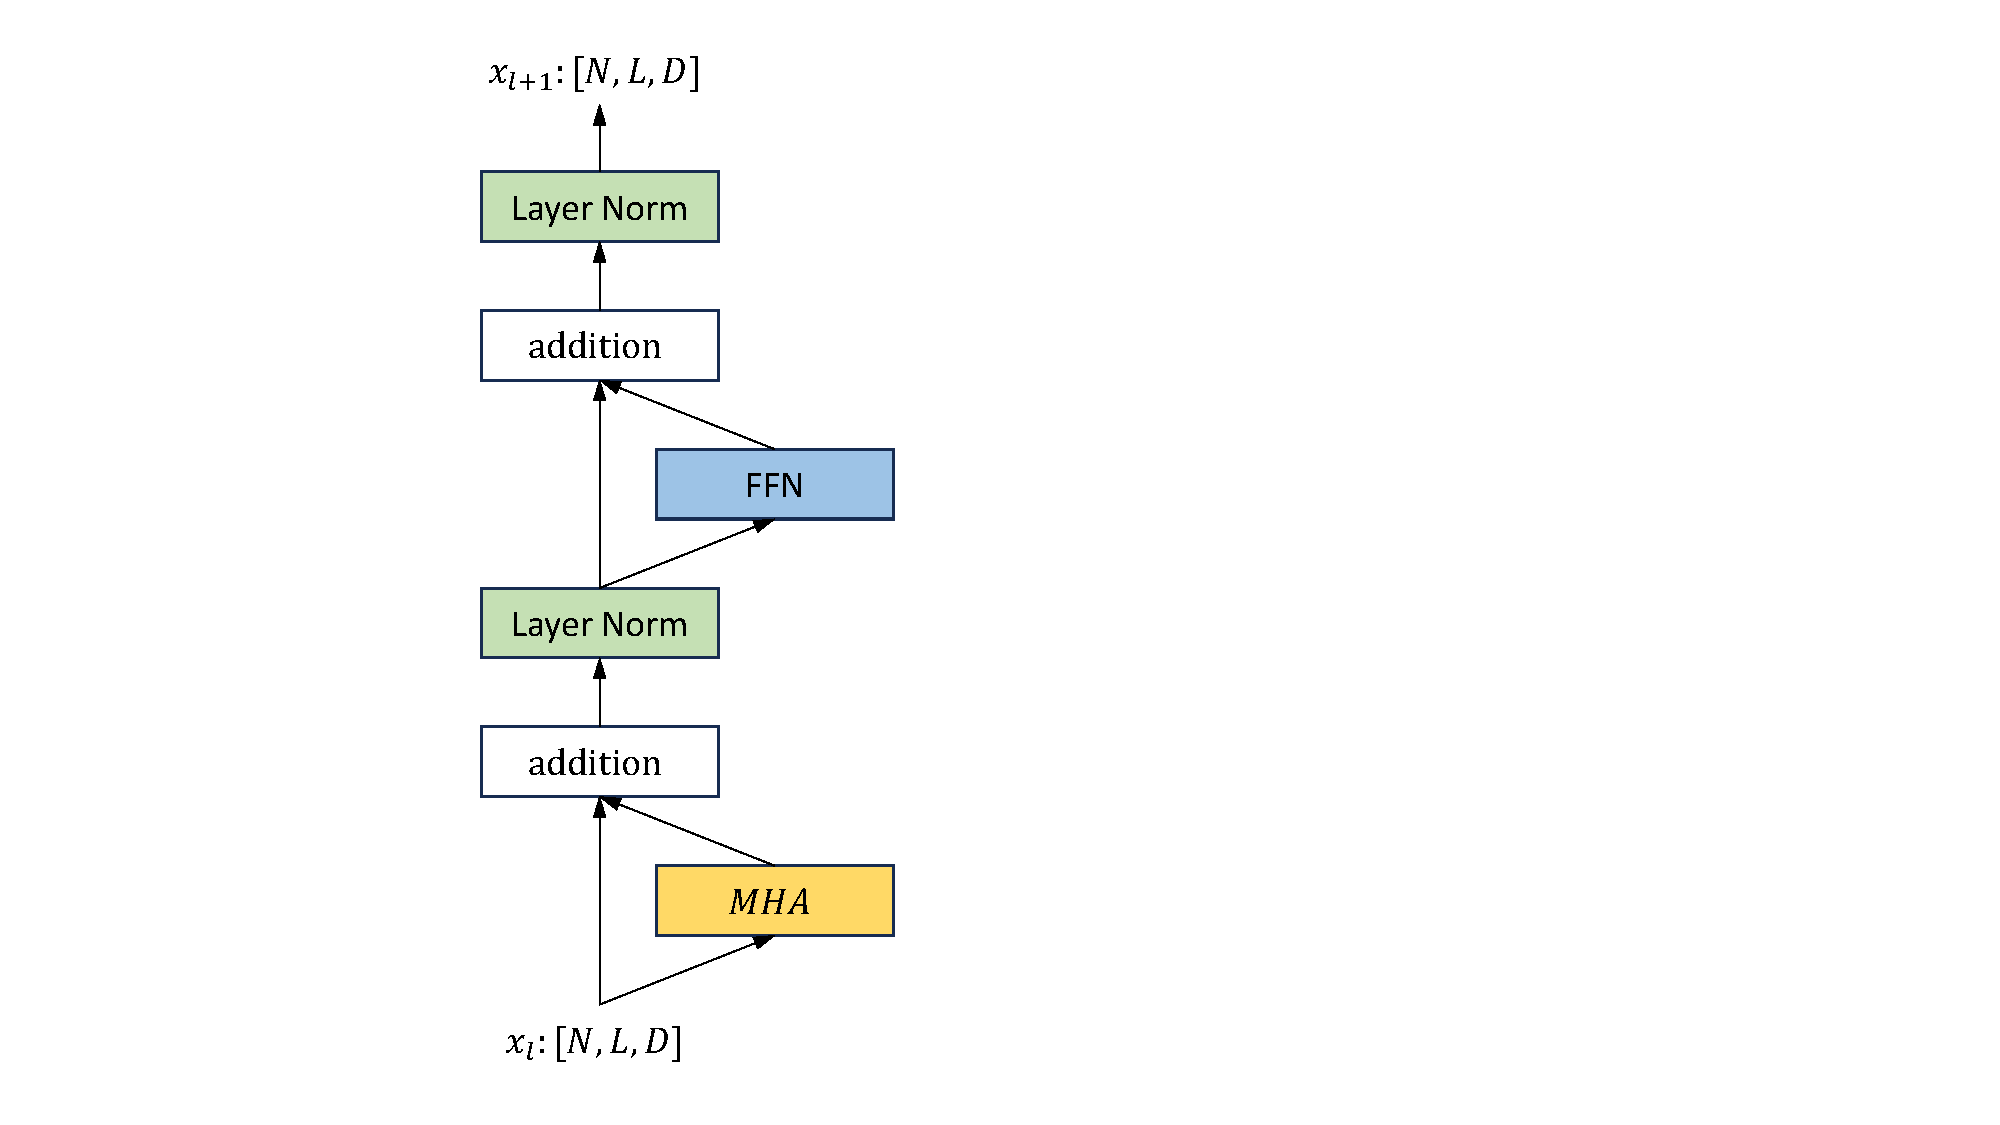
\includegraphics[width=3cm]{figures/Transformer-block.pdf}
    }
    \subfigure[Fused transformer block]{
    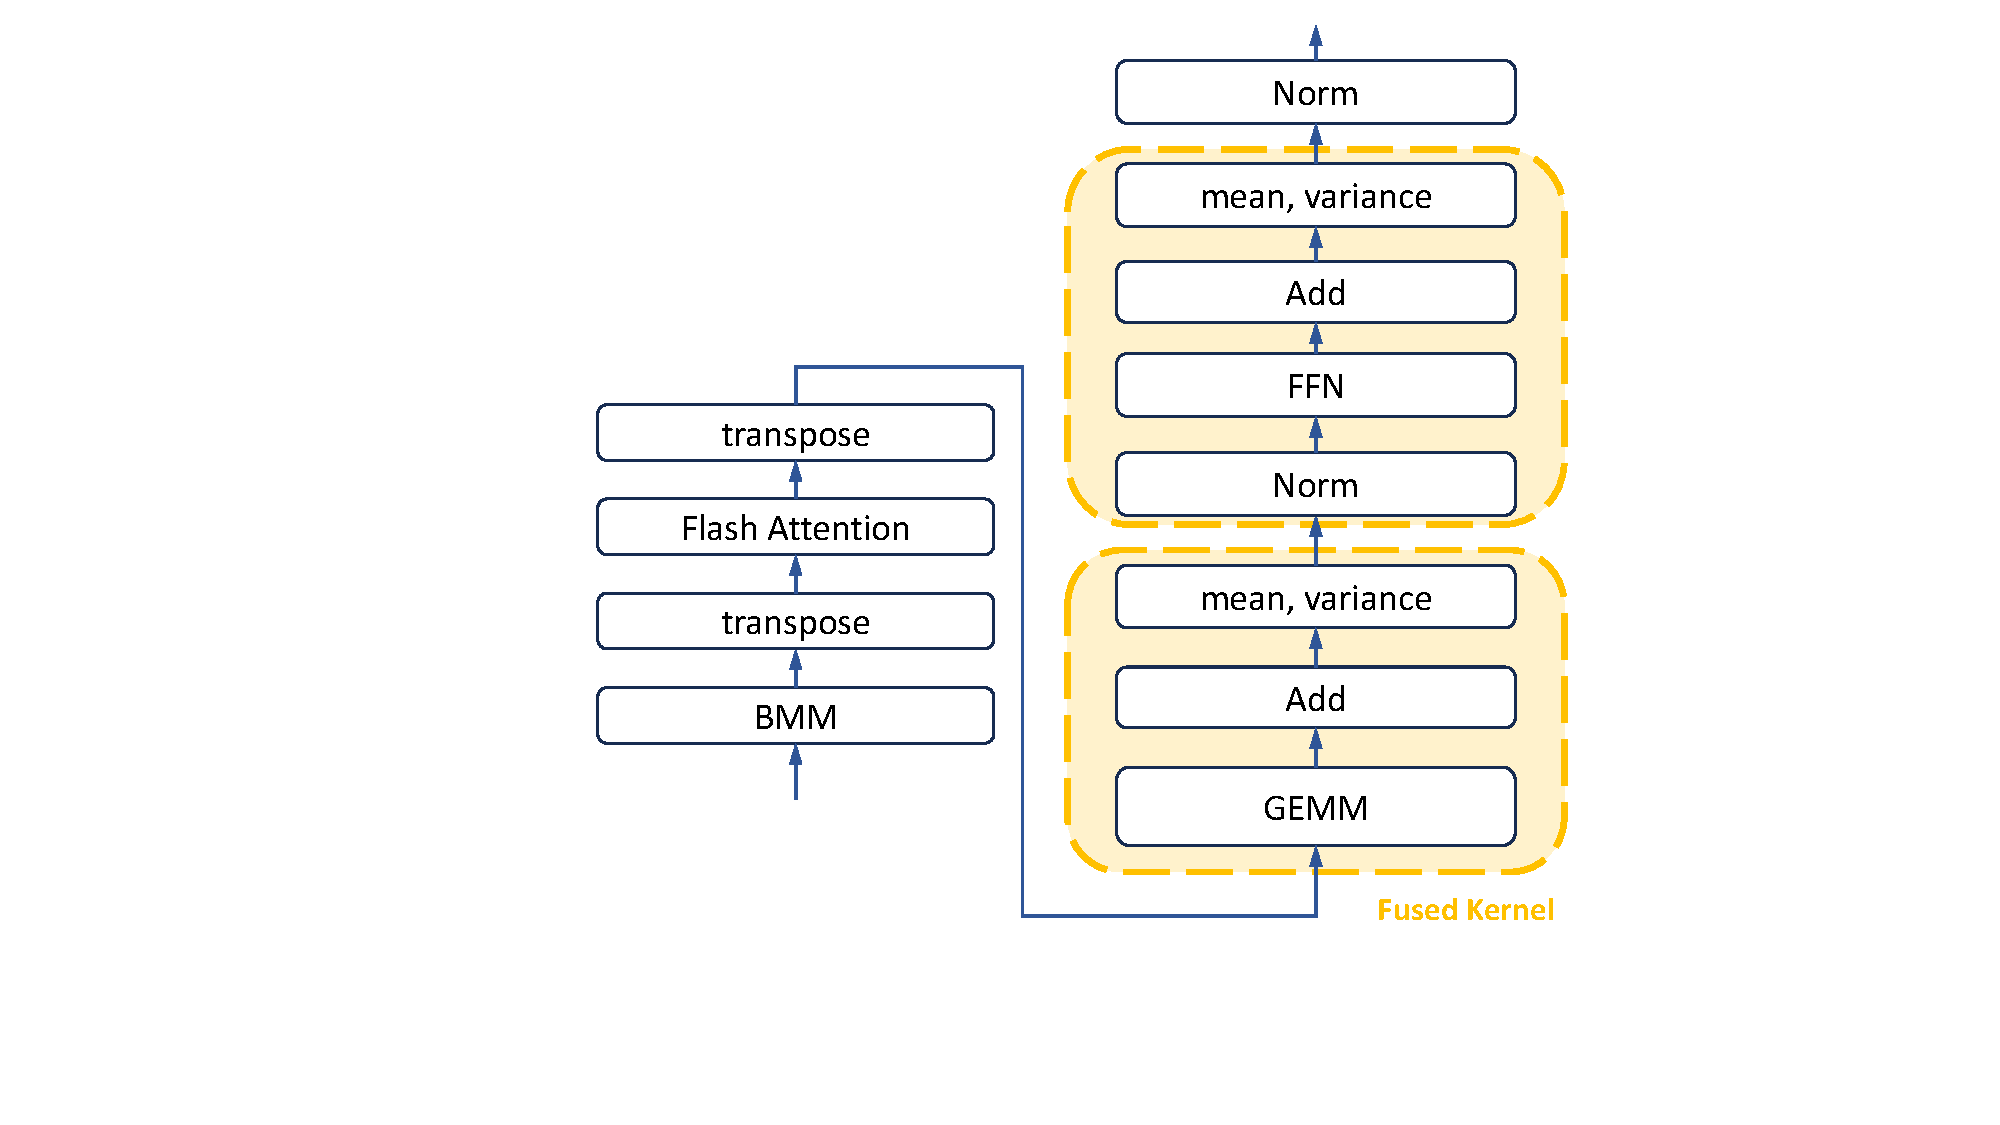
\includegraphics[width=7.5cm]{figures/fused_transformer_block.pdf}
    }
    \caption{Transformer block and a possible fusion plan.}\label{transformer-block}
\end{figure}
\vspace{-0.1cm}

The transformer model consists of a series of transformer blocks that are stacked on top of each other.
A transformer block is as shown above.

\subsection{MHA}

% \begin{align*}
% Q&=xW_q + b_q\\
% K&=xW_k + b_k\\
% V&=xW_v + b_v \\
% Q&=\text{transpose}(Q) \\
% K&=\text{transpose}(K) \\
% V&=\text{transpose}(V) \\
% O&=\text{softmax}(QK^T)V \\
% O&= \text{transpose}(O) \\
% O&=O W_o + b
% \end{align*}

\begin{figure}[h]
    \centering
    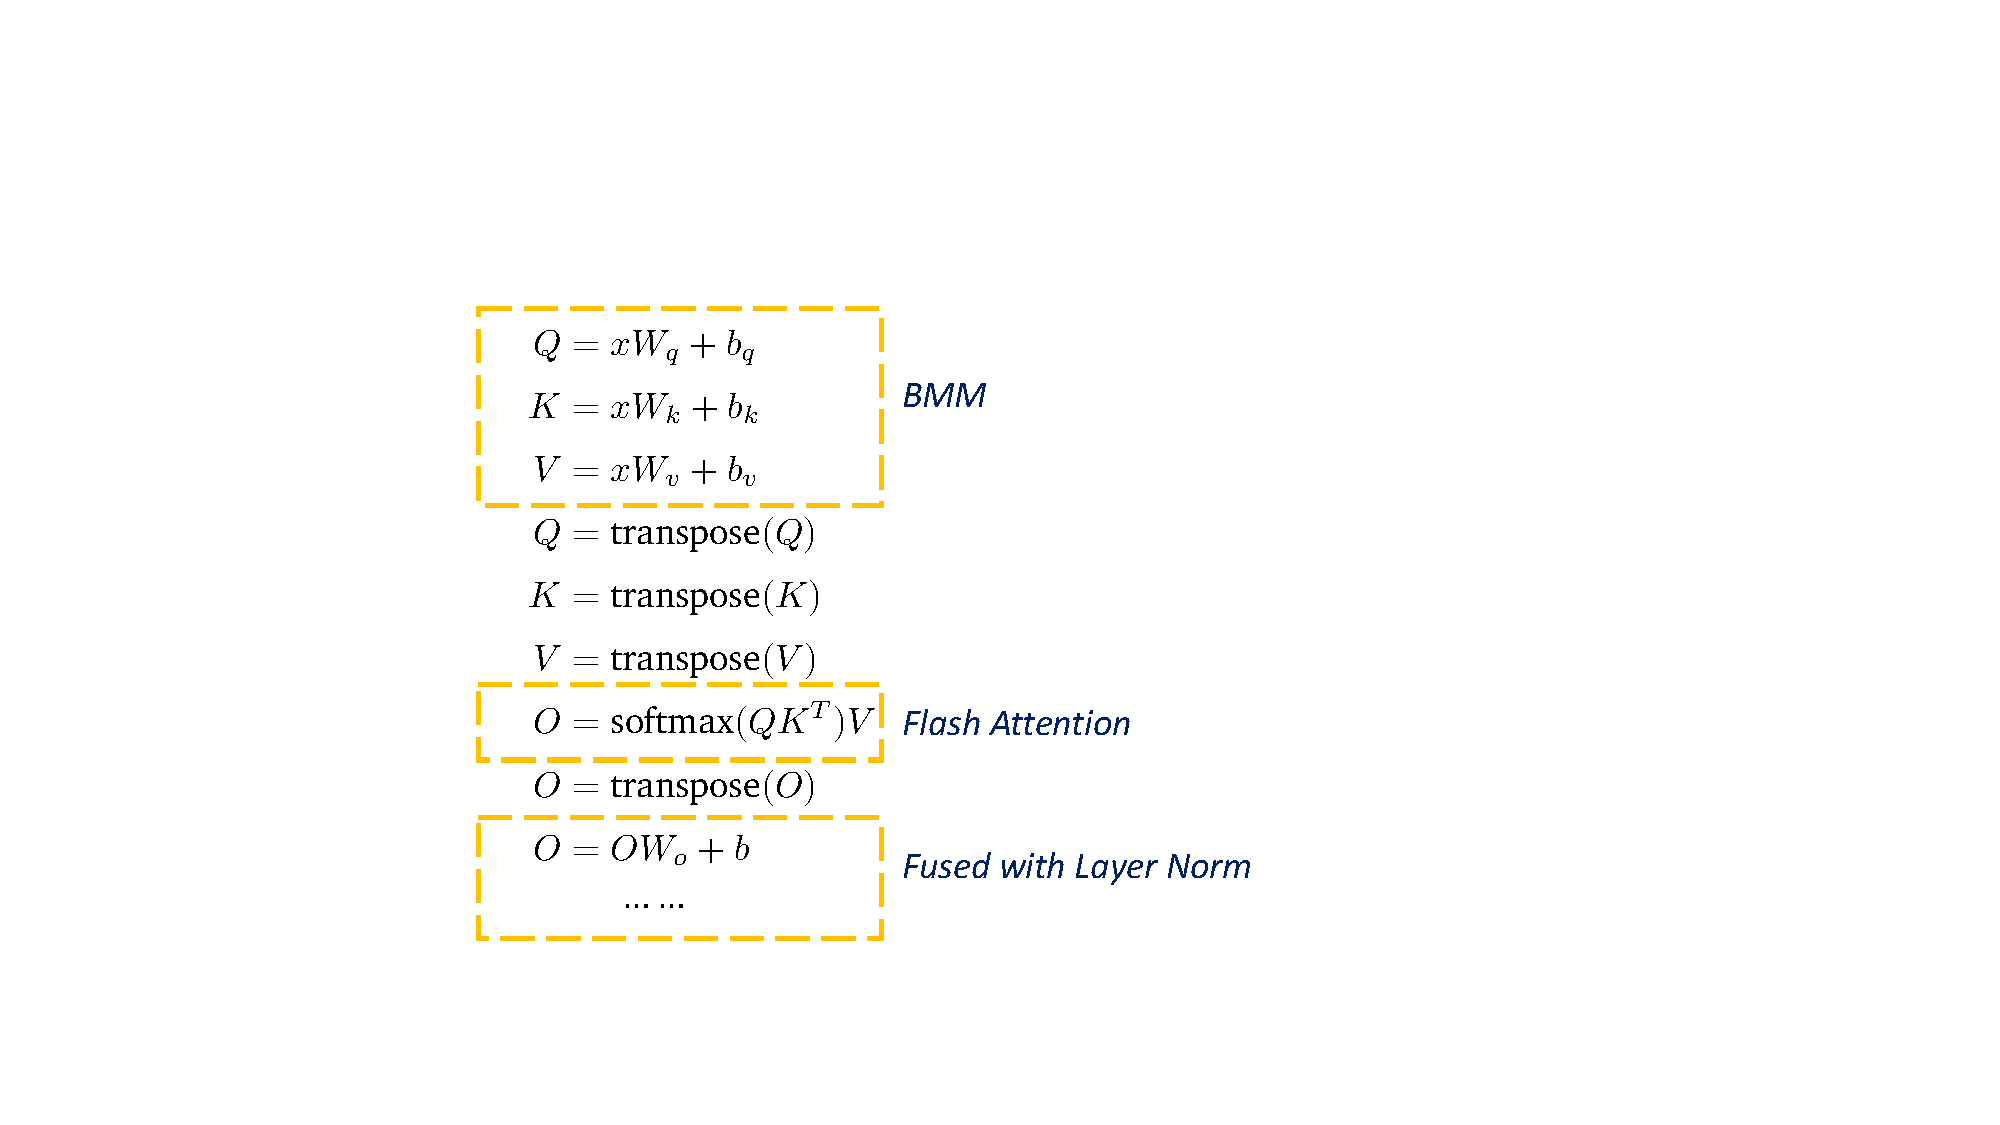
\includegraphics[width=0.4\textwidth]{figures/fused_mha.pdf}
    \caption{The fusion plan for MHA.}
\end{figure}

% \begin{table}[!htbp]
%     % \footnotesize
%     \setlength{\tabcolsep}{4pt}
%     \centering
%     \caption{Input tensors and their shapes.}
%     \begin{tabular}{c|l}
%     \textbf{Input}&\textbf{Shape} \\\midrule
%     $x \times W_Q$&$[N \times L, D] \times [D, D]$ \\
%     $x \times W_K$&$[N \times L, D] \times [D, D]$ \\
%     $x \times W_V$&$[N \times L, D] \times [D, D]$ \\
%     \end{tabular}
% \end{table}

\subsection{Layer Normalization}

$$y = \text{layernorm}(oW_o + b + x)$$

Input tensor $x$ has a shape of $N \times L \times D$ where $N$ stands for batch size, $L$ stands for sequence length, and $D$ stands for hidden size.
In the original Transformer, $D = 512$.

$$y_i=\frac{x_i-\mu}{\sqrt{\sigma^2 + \epsilon}}*\gamma_i+\beta_i\ \ \ i = [0, \ldots D-1]$$

Be definition:
\begin{align*}
    \mu_N &= \frac{1}{N}\sum_{i=1}^{N}x_i \\
    \sigma_{N}^2&=\frac{1}{N-1}\sum_{i=1}^{N}(x_i-\mu_{N})^2 \\
\end{align*}

To compute layer noramlization blockwise, we must use welford's online algorithm\cite{welford1962note} to compute the variance $\sigma^2$.
Define a quantity called $s_N = \sum^{N}_{i=1}(x_i - \mu_{N})^2$:

$$s_{N}=s_{N-1}+(x_N-\mu_{N-1})(x_N-\mu_N)$$

\subsection{FFN}

$W_1$ has a shape of $D \times 4D$ and $W_2$ has a shape of $4D * D$.

$$\text{FFN}(x) =\max(0, xW_1+b_1)W_2+b_2$$

\begin{align*}
\end{align*}

\subsection{Multi-scale Attention}

\begin{align*}
v_1 &= QK^T * \text{mask}\\
v_2 &= |v_1|.\text{sum}(\text{dim}=-1).\text{clamp}(\text{min}=1) \\
O &= \frac{v_1}{v_2}V  \\
\end{align*}

\begin{table}[!htbp]
    % \footnotesize
    \setlength{\tabcolsep}{4pt}
    \centering
    \caption{Input tensors and their shapes.}
    \begin{tabular}{c|c}
    \textbf{Input}&\textbf{Shape} \\\midrule
    $Q$ & $[N, H, L, E]$ \\
    $K$ & $[N, H, E, L]$ \\
    $V$ & $[N, H, L, E]$ \\
    $M$(mask) & $[H, L, L]$
    \end{tabular}
\end{table}

$N$ stands for batch size, $H$ stands for head number, $L$ stands for sequence length and $E$ stands for head dimensionality.

% \begin{lstlisting}[language=code_example, caption={}]
% for (:$i_1 \leftarrow [0, N-1)$:)  // batch size
%     for (:$i_2 \leftarrow [0, H-1)$:)  // number heads
%         for (:$i_3 \leftarrow [0, L-1)$:)  // sequence length
%             for (:$i_4 \leftarrow [0, L-1)$:)  // sequence length
%                 (:$v_1[i_4]=\text{\textbf{\textcolor{tomato}{dot}}}(Q[i_1, i_2, i_3],K[i_1, i_2, i_4])\textbf{\textcolor{tomato}{*}}\  M[i_2, i_3, i_4]$:)
%             (:$v_2 = $:)reduce(:($\textbf{\textcolor{tomato}{+}}, 0, \text{\textbf{\textcolor{tomato}{abs}}}(v_1))$:)
%             (:$O[i_1, i_2, i_3]=v_1V[i_1, i_2, i_3] \ \textbf{\textcolor{tomato}{/}}\ \textcolor{tomato}{\textbf{max}}(v_2, 1.)$:)  // [1, head_dim] x [head_dim, 1]
% \end{lstlisting}

\begin{figure}[h]
    \centering
    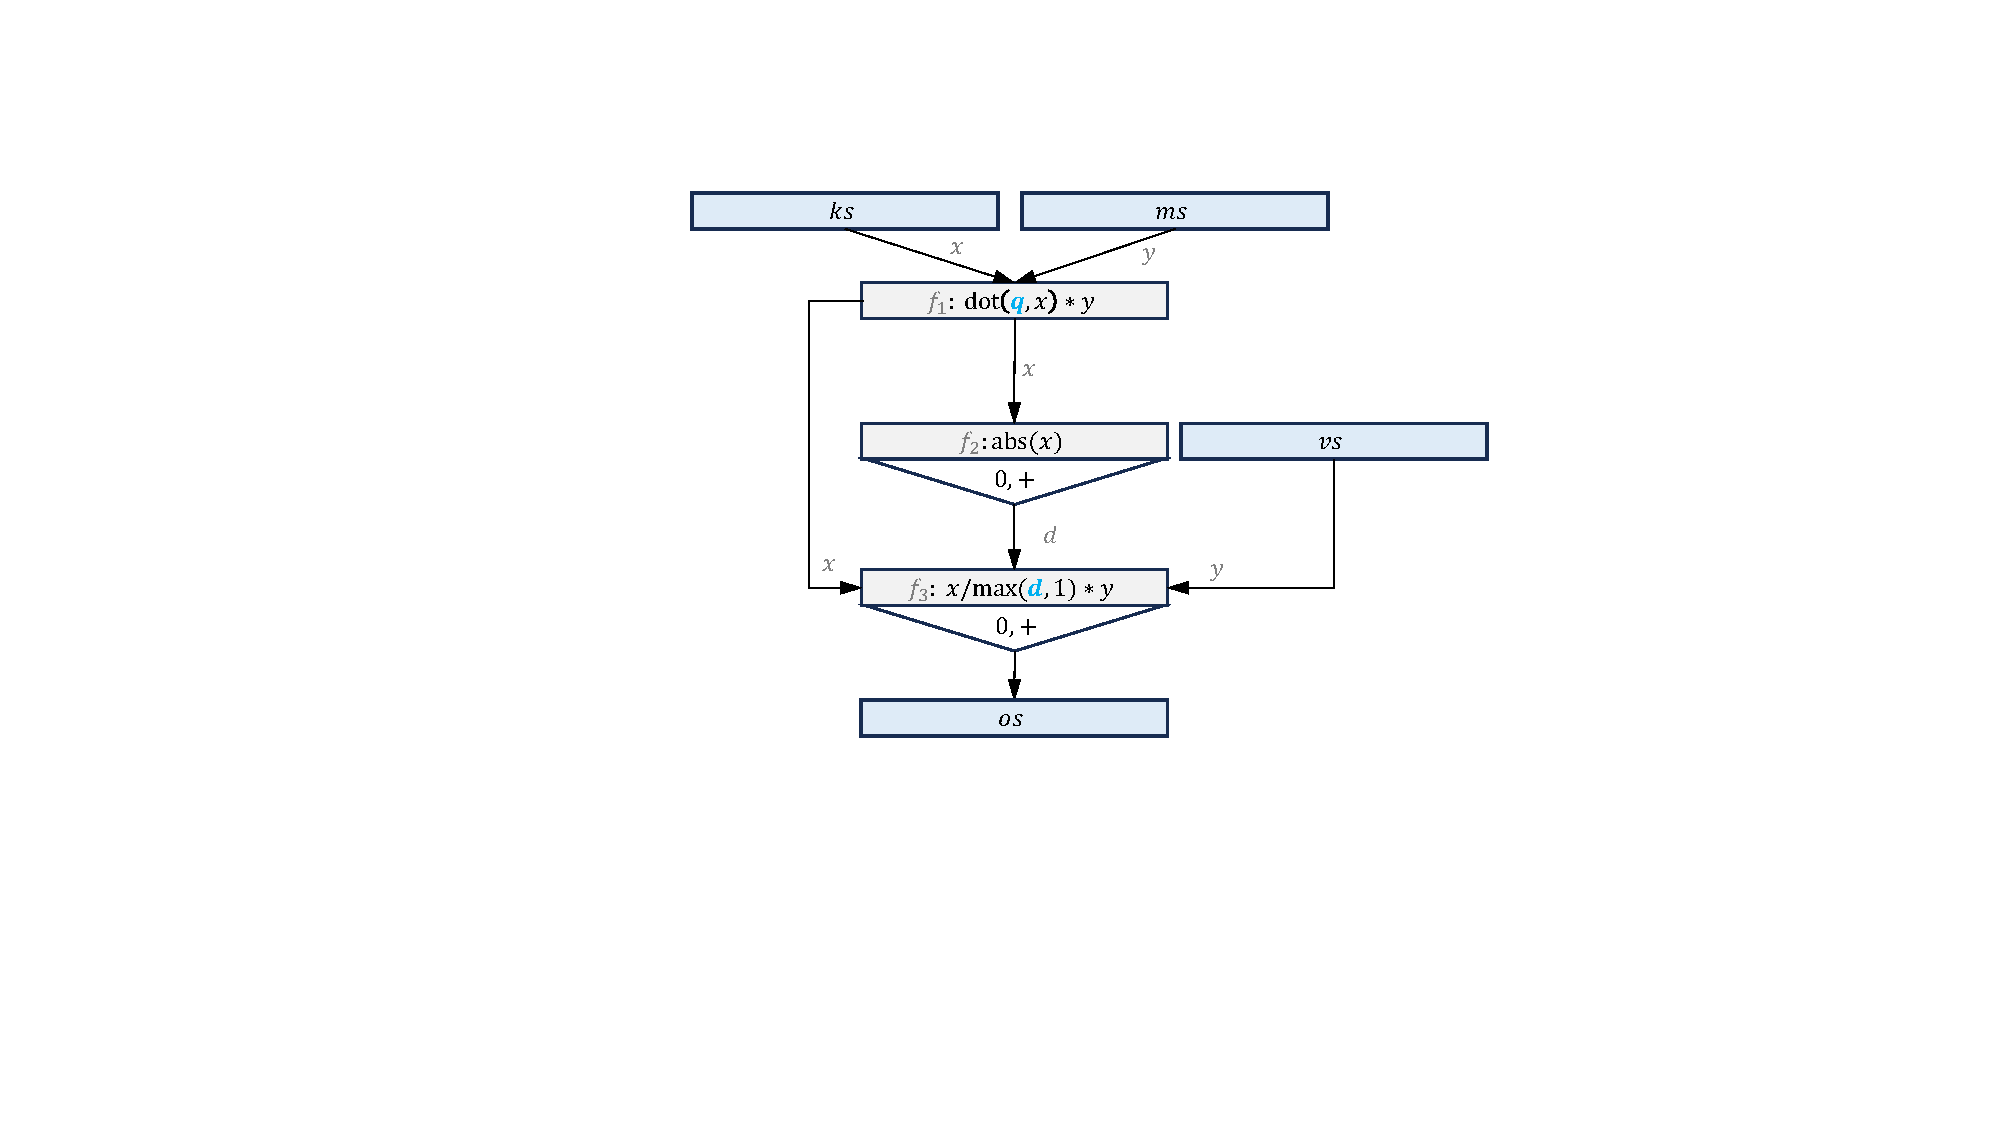
\includegraphics[width=0.65\textwidth]{figures/multi-scale-attn1.pdf}
    \caption{The multi-scale attention: the original computional flow.}
\end{figure}

\begin{figure}[h]
    \centering
    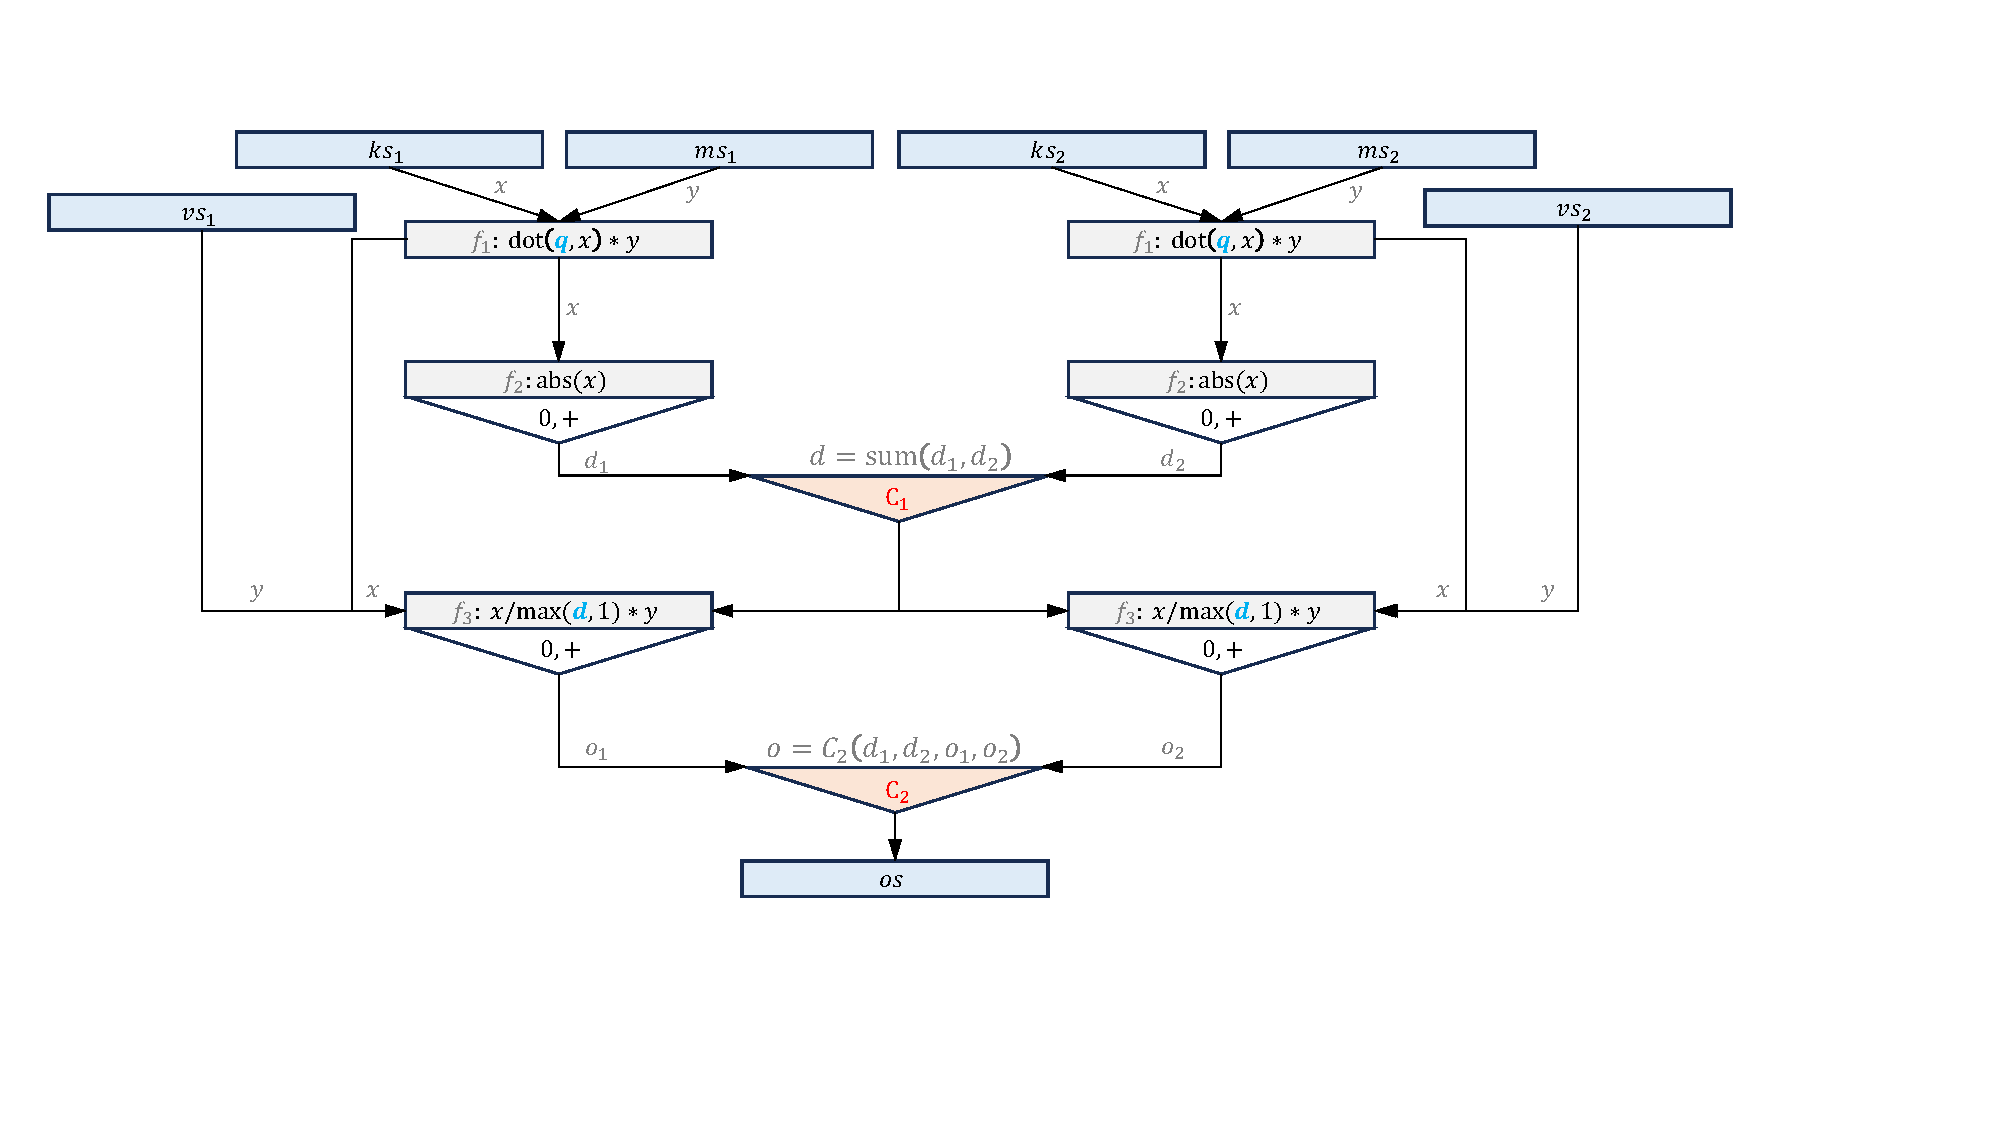
\includegraphics[width=1.\textwidth]{figures/multi-scale-attn2.pdf}
    \caption{The multi-scale attention: the expected computational flow.}
\end{figure}

$C_1$ is trivial:
$$C_1(d_1, d_2) = d_1+d_2$$

Consider $\bar{o}_1 = \frac{\bar{x}_1*\bar{y}_1}{d_1}$ has been computed for a single block, but a new constant $d'=\max(d_1, 1)$ has to be broadcast to the entire list $\bar{x}_1$ to compute a new output $\bar{o}_1'=\frac{\bar{x}_1*\bar{y}_1}{d_1'}$.

\begin{align*}
    \bar{x}_1*\bar{y}_1 &= d_1*\bar{o}_1 \\
    \bar{o}_1' &= \frac{\bar{x}_1*\bar{y}_1}{d'} = \frac{d_1 * \bar{o}_1}{d'}
\end{align*}

Similarly: $\bar{o}_2' = \frac{\bar{x}_2*\bar{y}_2}{d'} = \frac{d_2 * \bar{o}_2}{d'}$, therefore:

\begin{align*}
o&=\bar{o}_1'+\bar{o}_2' \\
&=\frac{1}{d'}(d_1*\bar{o}_1+d_2\bar{o}_2)
\end{align*}

\begin{align*}
\bar{v} &= [\bar{v}_1:\bar{v}_2] \\
r_1 &= \text{sum}(\bar{v}_1) & r_2 &= \text{sum}(\bar{v}_2) \\
d_1 &=\max(r_1, 1) &d_2 &= \max(r_2, 1) \\
\end{align*}

$\max(\text{sum}(r_1, r_2), 1) \ne \max(\text{sum}(\bar{v}), 1)$.

\textbf{Inputs}: $r_{i-1}:[B_r, 1]$,$d_{i-1}:[B_r,1]$, $o_{i}:[B_r, d]$, $q_i: [B_r, d]$, $k_i: [d, B_c]$, $v_i : [d, B_c]$, $m_i : [B_r, B_c]$

\textbf{Outputs}: $r_i:[B_r, 1]$, $d_{i}:[B_r, 1]$, $o_{i}:[B_r,d]$

\begin{lstlisting}[language=code_example, caption={Fused multi-scale attention kernel.}]
// o and d are accumulators
// q, k, v, m are input tiles
for (:$\textcolor{tomato}{r_{i-1}}, \textcolor{tomato}{d_{i-1}}, \textcolor{tomato}{o_{i-1}}, q_i, k_i, v_i, m_i \leftarrow i = [0, \frac{L}{B_c})$:) 
  // compute partial results for the current tile
  (:$t_i = q_i@k_i*m_i$:)
  (:$\bar{r}_i = \text{sum}(\text{abs}(t_i), \text{dim=-1}))$:)
  (:$o_{prev} = t_i@v_i$:)
  
  // update accumulators 
  (:$\bar{o}_i = d_{i-1} * o_{i-1} + o_{prev}$:)
  (:$\textcolor{tomato}{r_i} = r_{i-1} + \bar{r}_i$:)
  (:$\textcolor{tomato}{d_i} = \max(r_i, \mathbf{1}.)$:)
  (:$\textcolor{tomato}{o_i} = \bar{o}_i/d_i$:)
\end{lstlisting}